\begin{frame}
\frametitle{Two supported hardware platforms}
  There are two variants of the practical labs for this course, one
  supporting the Beaglebone Black board, the other supporting the
  STMicroelectronics STM32MP157A-DK1 Discovery board.
  \vfill
  \begin{columns}
    \column{0.5\textwidth}
    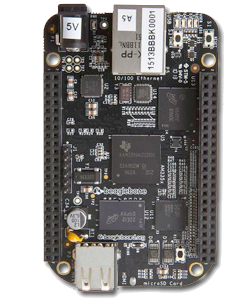
\includegraphics[height=0.5\textheight]{slides/beagleboneblack-board/beagleboneblack.png}
    \newline
    Beaglebone Black
    \newline {\scriptsize \url{https://bootlin.com/doc/training/yocto/}}
    \column{0.5\textwidth}
    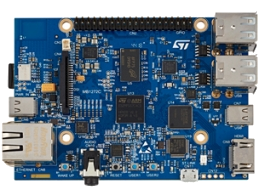
\includegraphics[height=0.5\textheight]{slides/discovery-board-dk1/discovery-board-dk1.png}
    \newline
    STM32MP157A-DK1 Discovery
    \newline {\scriptsize \url{https://bootlin.com/doc/training/yocto-stm32/}}
  \end{columns}
\end{frame}

\begin{frame}
\frametitle{Shopping list: hardware for this course}
  \begin{columns}
    \column{0.75\textwidth}
    \footnotesize
    \begin{itemize}
      \item Main board, choice 1:
      \begin{itemize}
        \item STMicroelectronics STM32MP157A-DK1 Discovery kit
        (Mouser: 65 EUR + VAT)
        \item USB-C cable (power supply)
        \item USB-A to micro B cable (serial console)
      \end{itemize}
      \item Main board, choice 2:
      \begin{itemize}
        \item Beaglebone Black or Beaglebone Black Wireless
        (Mouser: 73 EUR + VAT), USB-A to micro B power cable included
        \item USB Serial Cable - Female ends: \\
        Olimex: \url{https://j.mp/18Hk8yF}
      \end{itemize}
      \item Nintendo Nunchuk with UEXT connector: \\
            Olimex: \url{https://j.mp/1dTYLfs}
      \item Breadboard jumper wires - Male ends: \\
            Olimex: \url{https://bit.ly/2pSiIPs}
      \item SD card with 8 GB capacity
    \end{itemize}
    \column{0.25\textwidth}
    \includegraphics[height=0.25\textheight]{slides/using-either-bbb-or-stm32/nunchuk.jpg} \\
    \vspace{1cm}
    \includegraphics[height=0.15\textheight]{slides/using-either-bbb-or-stm32/jumper-wires.jpg} \\
    \vspace{1cm}
    %% Source: https://commons.wikimedia.org/wiki/File:SD_card_icon.svg
    \includegraphics[height=0.15\textheight]{slides/using-either-bbb-or-stm32/sd-card.pdf}
  \end{columns}
\end{frame}
